\documentclass[journal,twoside,web]{ieeecolor}
\usepackage{tmi}
\usepackage{amsmath,amssymb,amsfonts}
\usepackage{algorithmic}
\usepackage{graphicx}
\graphicspath{{images}}
\usepackage{textcomp}
\def\BibTeX{{\rm B\kern-.05em{\sc i\kern-.025em b}\kern-.08em
    T\kern-.1667em\lower.7ex\hbox{E}\kern-.125emX}}
\markboth{\journalname, VOL. XX, NO. XX, XXXX 2020}
{Author \MakeLowercase{\textit{et al.}}: Preparation of Papers for IEEE TRANSACTIONS ON MEDICAL IMAGING}
\begin{document}
\title{Verarbeitung von Gesichtsaufnahmen zur Genderklassifikation als Anwendung neuronaler Netze}
\author{Gruppe: Niklas Herrhofer, Celine Schneider, Andreas Braig\IEEEmembership{TEL22AT1},
\thanks{This paragraph of the first footnote will contain the date on which
you submitted your paper for review. It will also contain support information,
including sponsor and financial support acknowledgment. For example, 
``This work was supported in part by the U.S. Department of Commerce under Grant BS123456.'' }
\thanks{The next few paragraphs should contain the authors' current affiliations,
including current address and e-mail. For example, F. A. Author is with the
National Institute of Standards and Technology, Boulder, CO 80305 USA (e-mail:author@boulder.nist.gov). }
\thanks{S. B. Author, Jr., was with Rice University, Houston, TX 77005 USA.
He is now with the Department of Physics, Colorado State University,
Fort Collins, CO 80523 USA (e-mail: author@lamar.colostate.edu).}
\thanks{T. C. Author is with the Electrical Engineering Department,
University of Colorado, Boulder, CO 80309 USA, on leave from the National
Research Institute for Metals, Tsukuba, Japan (e-mail: author@nrim.go.jp).}}

\maketitle

\begin{abstract}
    Brauchen wir echt ein Abstract? 
\end{abstract}


\begin{IEEEkeywords}
    Neuronales Netz, Bildsegmentierung, Convolutional Neural Network, 
\end{IEEEkeywords}

\section{Problemstellung und Ziel dieser Arbeit}
\label{sec:introduction}
\IEEEPARstart{D}{iese} Arbeit befasst sich Mit der Verarbeitung und Klassifikation einzelner Datenpunkte in einem Datensatz.
Die hierbei verwendeten Daten sind Gesichtsaufnahmen verschiedener Personen verschiedenen Alters. 

Die erste Teilaufgabe besteht in der Segmentierung und Verarbeitung dieses bereitgestellten Datensatzes, um die Gesichtselemente einheitlich im Bild zu positionieren. 
Augen und Mund sollen hierbei immer ein gleichschenkliges Dreieck an einer festen Position im Bild bilden. 

Die zweite Teilaufgabe befasst sich mit dem Klassifikationsproblem. 
Der verarbeitete Datensatz wird in ein Convolutional Neural Network geladen und das Geschlecht der abgebildeten Person klassifiziert. 
Hierbei soll das Netz eine binäre Klassifikation zwischen Männlich (0) und Weiblich (1) durchführen.

Für die Lösung dieser Aufgabe wurde die Programmiersprache Python mit den wesentlichen Bibliotheken "OpenCV", "numpy" und "Pytorch" verwendet. 

\section{Stand der Technik}
In diesem Kapitel wird der aktuelle Stand der Technik zur Bildsegmentierung und Klassifizierung Diskutiert.

\subsection{Python}
Define abbreviations and acronyms the first time they are used in the text, 
even after they have already been defined in the abstract. Abbreviations 
such as IEEE, SI, ac, and dc do not have to be defined. Abbreviations that 
incorporate periods should not have spaces: write ``C.N.R.S.,'' not ``C. N. 
R. S.'' Do not use abbreviations in the title unless they are unavoidable 
(for example, ``IEEE'' in the title of this article).

\subsection{Klassifikationsprobleme}
Use one space after periods and colons. Hyphenate complex modifiers: 
``zero-field-cooled magnetization.'' Avoid dangling participles, such as, 
``Using \eqref{eq}, the potential was calculated.'' It is not clear who or what 
used \eqref{eq}. Write instead, ``The potential was calculated by using \eqref{eq},'' or 
``Using \eqref{eq}, we calculated the potential.''

Use a zero before decimal points: ``0.25,'' not ``.25.'' Use 
``cm$^{3}$,'' not ``cc.'' Indicate sample dimensions as ``0.1 cm 
$\times $ 0.2 cm,'' not ``0.1 $\times $ 0.2 cm$^{2}$.'' The 
abbreviation for ``seconds'' is ``s,'' not ``sec.'' Use 
``Wb/m$^{2}$'' or ``webers per square meter,'' not 
``webers/m$^{2}$.'' When expressing a range of values, write ``7 to 
9'' or ``7--9,'' not ``7$\sim $9.''

A parenthetical statement at the end of a sentence is punctuated outside of 
the closing parenthesis (like this). (A parenthetical sentence is punctuated 
within the parentheses.) In American English, periods and commas are located within 
quotation marks, like ``this period.'' Other punctuation is placed ``outside''! 
Avoid contractions; for example, write ``do not'' instead of ``don't.'' The 
serial comma is preferred: ``A, B, and C'' instead of ``A, B and C.''

If you wish, you may write in the first person singular or plural form using
the active voice (``I observed that $\ldots$'' or ``We observed that $\ldots$'' 
instead of ``It was observed that $\ldots$''). Remember to check spelling. If 
your native language is not English, please have a native English-speaking 
colleague to carefully proofread your paper.

\section{Der Datensatz}
In diesem Kapitel wird der verwendete Datensatz vorgestellt. Es soll nachvollziehbar sein welche Herausforderungen bei der Arbeit mit diesen Daten auftreten. 
\subsection{}
Number equations consecutively with equation numbers in parentheses flush 
with the right margin, as appears in \eqref{eq}. Refer to ``\eqref{eq},'' not ``Eq. \eqref{eq}'' 
or ``equation \eqref{eq},'' except at the beginning of a sentence: ``Equation \eqref{eq} 
is $\ldots$ .'' To make your equations more 
compact, you may use the solidus (~/~), the exp function, or appropriate 
exponents. Use parentheses to avoid ambiguities in denominators. Punctuate 
equations when they are part of a sentence, as in
\begin{equation}E=mc^2.\label{eq}\end{equation}

Be sure to define the symbols in your equation before the equation appears or
immediately following. Italicize symbols ($T$ might refer 
to temperature, but T is the unit tesla).

\subsection{\LaTeX-Specific Advice}

Use ``soft'' (e.g., \verb|\eqref{Eq}|) cross references instead
of ``hard'' references (e.g., \verb|(1)|). This will make it possible
to combine sections, add equations, or change the order of figures or
citations without having to manually change equation references.

Do not use the \verb|{eqnarray}| equation environment. Use
\verb|{align}| or \verb|{IEEEeqnarray}| instead. The \verb|{eqnarray}|
environment leaves unsightly spaces around relation symbols.

Note that the \verb|{subequations}| environment in {\LaTeX}
will increment the main equation counter even when there are no
equation numbers displayed.

{\BibTeX} only functions in conjunction with local .bib files. If you use {\BibTeX} to produce the
bibliography you must attach the .bib files.

{\LaTeX} can't read your mind. If you assign the same label to both a
subsubsection and a table, you may find that Table I has been cross
referenced as Table IV-B3. 

{\LaTeX} does not have precognitive abilities. If you put a
\verb|\label| command before the command that updates the counter it's
supposed to be using, the label will pick up the last counter to be
cross referenced instead. In particular, a \verb|\label| command
should not go before the caption of a figure or a table.

Do not use \verb|\nonumber| inside the \verb|{array}| environment. It
will not stop equation numbers inside \verb|{array}| and it might stop a
wanted equation number in the surrounding equation.

If you are submitting your paper to a colorized journal, you can use
the following two lines at the start of the article to ensure its
appearance resembles the final copy:

\smallskip\noindent
\begin{small}
\begin{tabular}{l}
\verb+\+\texttt{documentclass[journal,twoside,web]\{ieeecolor\}}\\
\verb+\+\texttt{usepackage\{\textit{Journal\_Name}\}}
\end{tabular}
\end{small}

\section{Units}
Use either SI (MKS) or CGS as primary units. (SI units are strongly 
encouraged.) English units may be used as secondary units (in parentheses). 
For example, write ``1 kg (2.2lb).'' An exception exists for when 
English units are used as identifiers in commercial products, such as a ``3\textonehalf-in 
disk drive.'' Avoid combining SI and CGS units, such as current in amperes 
and magnetic field in oersteds. This often leads to confusion because 
equations do not balance dimensionally. If you must use mixed units, clearly 
state the units for each quantity in an equation.

The SI unit for magnetic field strength $H$ is A/m. However, if you wish to use 
units of T, either refer to magnetic flux density $B$ or magnetic field 
strength symbolized as $\mu _{0}H$. Use the center dot to separate 
compound units, e.g., ``A$\cdot $m$^{2}$.''

\begin{figure}[!t]
\centerline{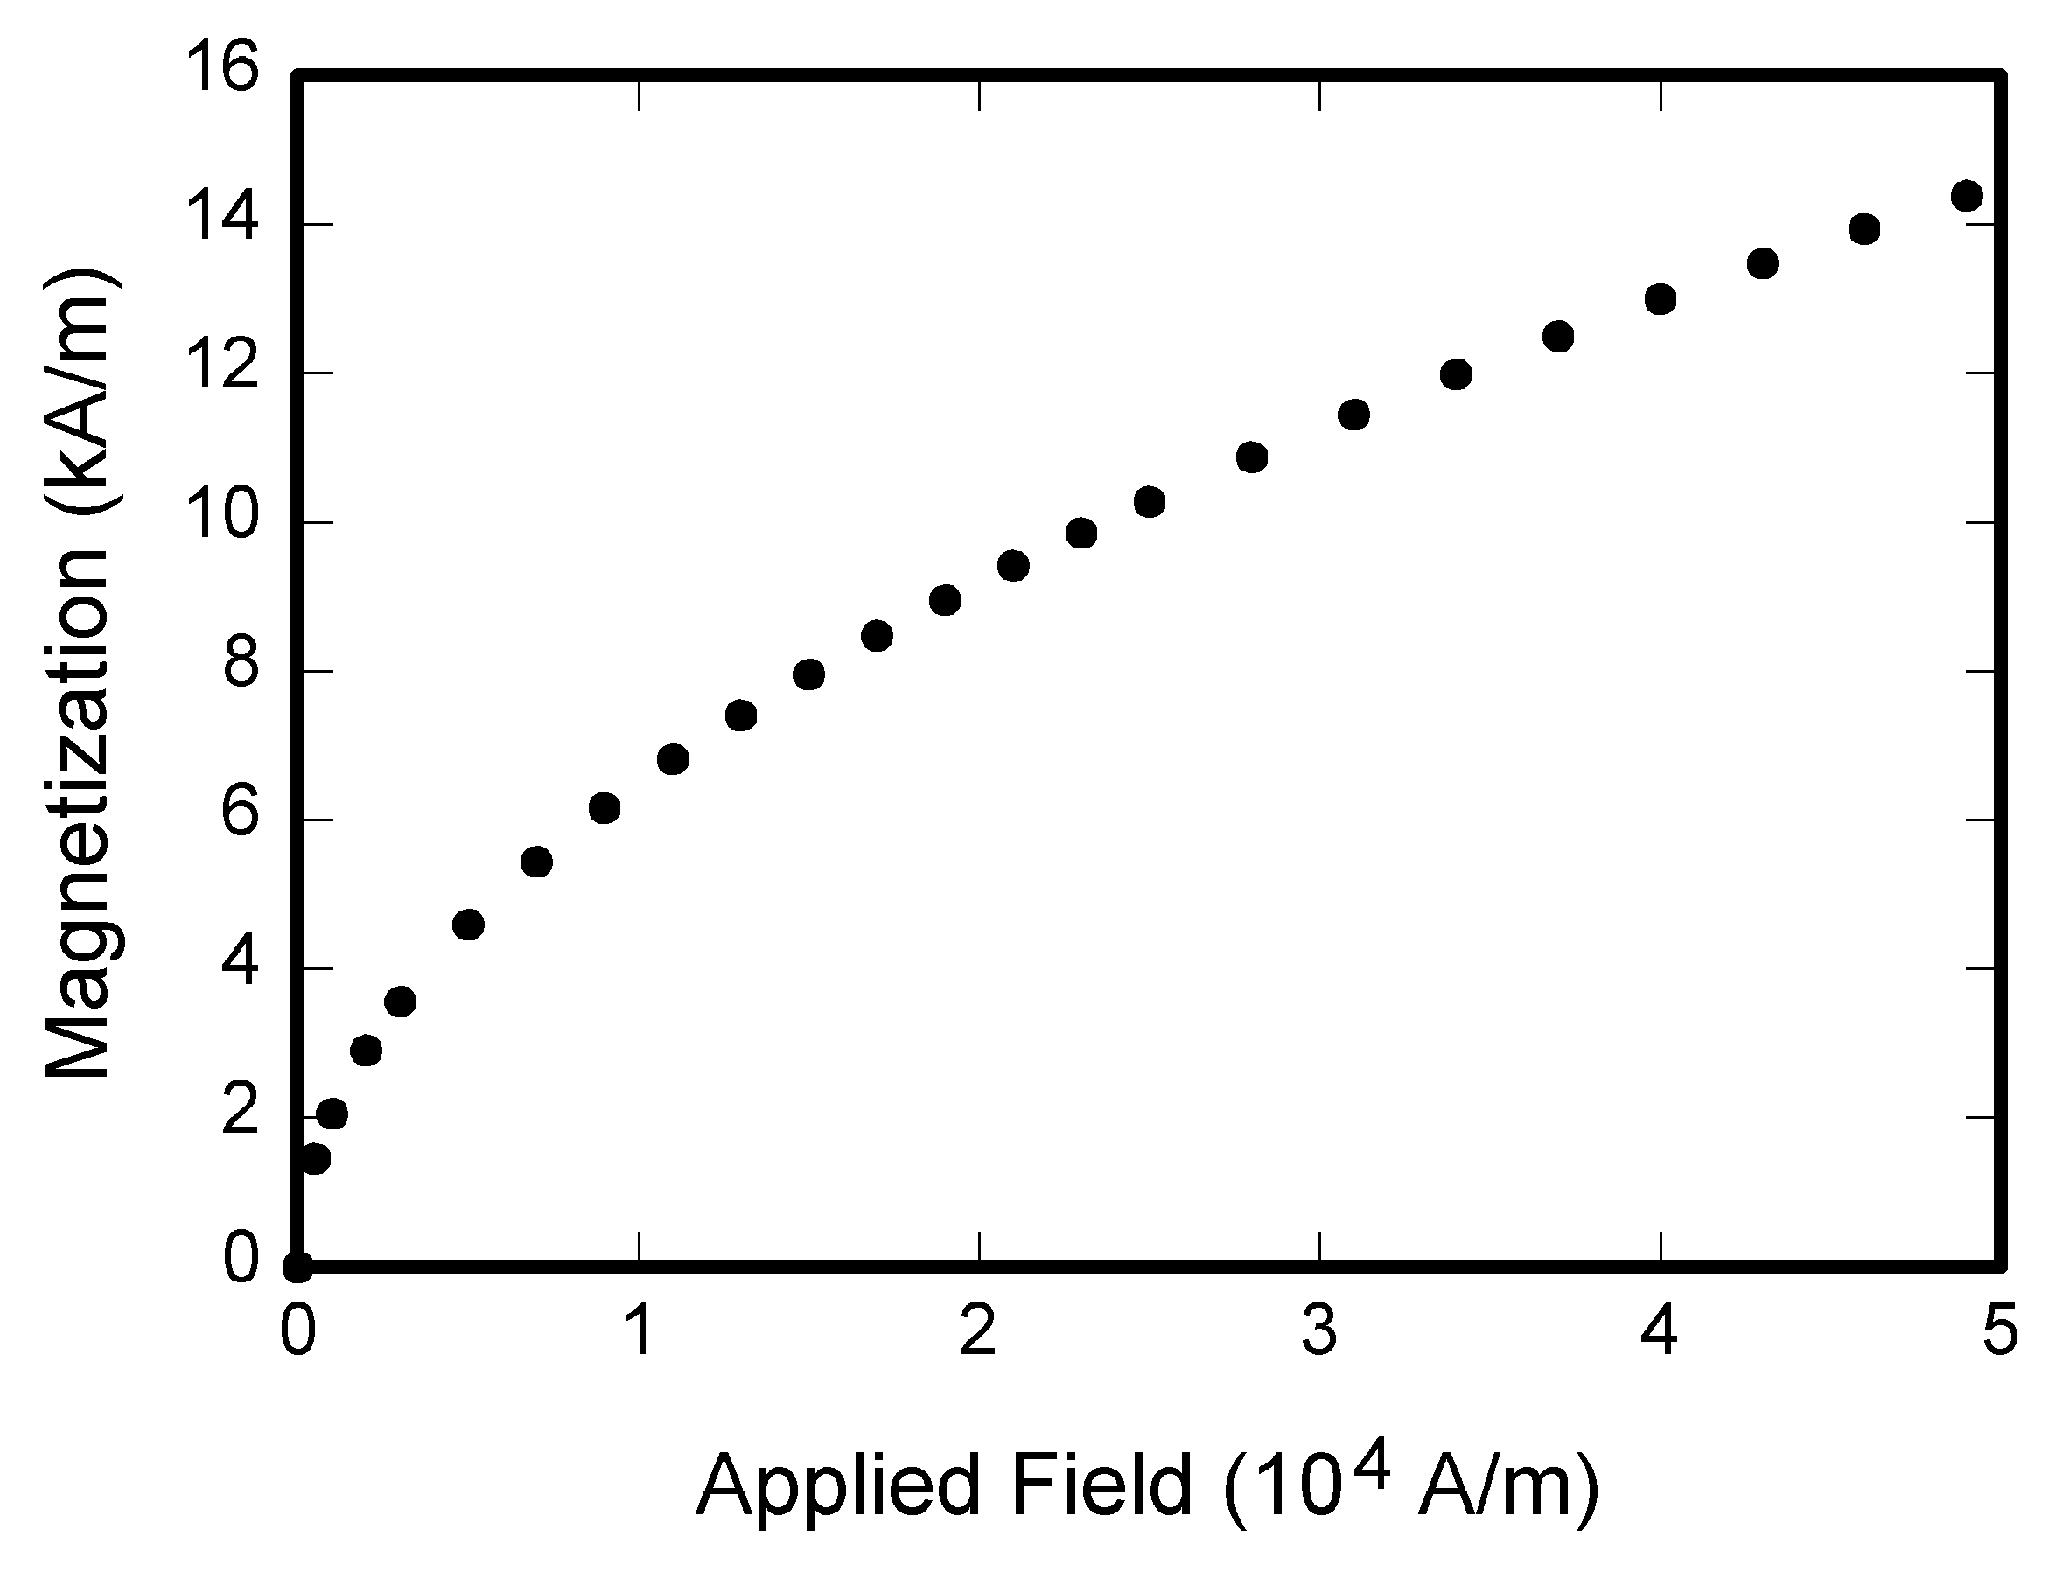
\includegraphics[width=\columnwidth]{fig1.png}}
\caption{Magnetization as a function of applied field.
It is good practice to explain the significance of the figure in the caption.}
\label{fig1}
\end{figure}

\section{Guidelines for Graphics Preparation and Submission}
\label{sec:guidelines}

\subsection{Types of Graphics}
The following list outlines the different types of graphics published in 
IEEE journals. They are categorized based on their construction, and use of 
color~/~shades of gray:

\subsubsection{Color/Grayscale figures}
{Figures that are meant to appear in color, or shades of black/gray. Such 
figures may include photographs, illustrations, multicolor graphs, and 
flowcharts.}

\subsubsection{Line Art figures}
{Figures that are composed of only black lines and shapes. These figures 
should have no shades or half-tones of gray, only black and white.}

\subsubsection{Author photos}
{Not allowed for papers in TMI.}

\subsubsection{Tables}
{Data charts which are typically black and white, but sometimes include 
color.}

\begin{table}
\caption{Units for Magnetic Properties}
\label{table}
\setlength{\tabcolsep}{3pt}
\begin{tabular}{|p{25pt}|p{75pt}|p{115pt}|}
\hline
Symbol& 
Quantity& 
Conversion from Gaussian and \par CGS EMU to SI $^{\mathrm{a}}$ \\
\hline
$\Phi $& 
magnetic flux& 
1 Mx $\to  10^{-8}$ Wb $= 10^{-8}$ V$\cdot $s \\
$B$& 
magnetic flux density, \par magnetic induction& 
1 G $\to  10^{-4}$ T $= 10^{-4}$ Wb/m$^{2}$ \\
$H$& 
magnetic field strength& 
1 Oe $\to  10^{3}/(4\pi )$ A/m \\
$m$& 
magnetic moment& 
1 erg/G $=$ 1 emu \par $\to 10^{-3}$ A$\cdot $m$^{2} = 10^{-3}$ J/T \\
$M$& 
magnetization& 
1 erg/(G$\cdot $cm$^{3}) =$ 1 emu/cm$^{3}$ \par $\to 10^{3}$ A/m \\
4$\pi M$& 
magnetization& 
1 G $\to  10^{3}/(4\pi )$ A/m \\
$\sigma $& 
specific magnetization& 
1 erg/(G$\cdot $g) $=$ 1 emu/g $\to $ 1 A$\cdot $m$^{2}$/kg \\
$j$& 
magnetic dipole \par moment& 
1 erg/G $=$ 1 emu \par $\to 4\pi \times  10^{-10}$ Wb$\cdot $m \\
$J$& 
magnetic polarization& 
1 erg/(G$\cdot $cm$^{3}) =$ 1 emu/cm$^{3}$ \par $\to 4\pi \times  10^{-4}$ T \\
$\chi , \kappa $& 
susceptibility& 
1 $\to  4\pi $ \\
$\chi_{\rho }$& 
mass susceptibility& 
1 cm$^{3}$/g $\to  4\pi \times  10^{-3}$ m$^{3}$/kg \\
$\mu $& 
permeability& 
1 $\to  4\pi \times  10^{-7}$ H/m \par $= 4\pi \times  10^{-7}$ Wb/(A$\cdot $m) \\
$\mu_{r}$& 
relative permeability& 
$\mu \to \mu_{r}$ \\
$w, W$& 
energy density& 
1 erg/cm$^{3} \to  10^{-1}$ J/m$^{3}$ \\
$N, D$& 
demagnetizing factor& 
1 $\to  1/(4\pi )$ \\
\hline
\multicolumn{3}{p{251pt}}{Vertical lines are optional in tables. Statements that serve as captions for 
the entire table do not need footnote letters. }\\
\multicolumn{3}{p{251pt}}{$^{\mathrm{a}}$Gaussian units are the same as cg emu for magnetostatics; Mx 
$=$ maxwell, G $=$ gauss, Oe $=$ oersted; Wb $=$ weber, V $=$ volt, s $=$ 
second, T $=$ tesla, m $=$ meter, A $=$ ampere, J $=$ joule, kg $=$ 
kilogram, H $=$ henry.}
\end{tabular}
\label{tab1}
\end{table}

\subsection{Multipart figures}
Multipart figures are comprised of more than one sub-figure presented together.
If a multipart figure is made up of multiple figure types (one part is lineart,
and another is grayscale or color) the figure should meet the strictest applicable guidelines.

\subsection{File Formats For Graphics}
\label{formats}
Format and save your graphics as one of the following approved file types:
PostScript (.PS), Encapsulated PostScript (.EPS), Tagged Image File Format (.TIFF),
Portable Document Format (.PDF), Portable Network Graphics (.PNG), or Metapost (.MPS).
After the paper is accepted, any included graphics must be submitted alongside the final manuscript files.

\subsection{Sizing of Graphics}
Most charts, graphs, and tables are one column wide (3.5 inches~/~88 
millimeters) or page wide (7.16 inches~/~181 millimeters). The maximum
depth of a graphic is 8.5 inches (216 millimeters). When choosing the depth of a graphic,
please allow space for a caption. Authors are allowed to size figures between column and
page widths, but it is recommended not to size figures less than column width unless necessary. 

\subsection{Resolution}
The proper resolution of your figures will depend on the type of figure it 
is as defined in the ``Types of Figures'' section. Author photographs, 
color, and grayscale figures should be at least 300dpi. Lineart, including 
tables should be a minimum of 600dpi.

\subsection{Vector Art}
While IEEE does accept and even recommends that authors submit artwork
in vector format, it is our policy is to rasterize all figures for publication. This is done
in order to preserve figures' integrity across multiple computer platforms.

\subsection{Colorspace}
The term colorspace refers to the entire sum of colors that can be 
represented within a given medium. For our purposes, the three main colorspaces
are grayscale, RGB (red/green/blue) and CMYK (cyan/magenta/yellow/black).
RGB is generally used with on-screen graphics, whereas CMYK is used for printing purposes.

All color figures should be generated in RGB or CMYK colorspace. Grayscale 
images should be submitted in grayscale colorspace. Line art may be 
provided in grayscale OR bitmap colorspace. Note that ``bitmap colorspace'' 
and ``bitmap file format'' are not the same thing. When bitmap colorspace 
is selected, .TIF/.TIFF are the recommended file formats.

\subsection{Accepted Fonts Within Figures}
When preparing your graphics IEEE suggests that you use of one of the 
following Open Type fonts: Times New Roman, Helvetica, Arial, Cambria, and 
Symbol. If you are supplying EPS, PS, or PDF files all fonts must be 
embedded. Some fonts may only be native to your operating system; without 
the fonts embedded, parts of the graphic may be distorted or missing.

A safe option when finalizing your figures is to strip out the fonts before 
you save the files, creating ``outline'' type. This converts fonts to 
artwork that will appear uniformly on any screen.

\subsection{Using Labels Within Figures}

\subsubsection{Figure Axis labels}
Figure axis labels are often a source of confusion. Use words rather than 
symbols. As an example, write the quantity ``Magnetization,'' or 
``Magnetization M,'' not just ``M.'' Put units in parentheses. Do not label 
axes only with units. As in Fig. 1, for example, write ``Magnetization 
(A/m)'' or ``Magnetization (A$\cdot$m$^{-1}$),'' not just ``A/m.''
Do not label axes with a ratio of quantities and units.
For example, write ``Temperature (K),'' not ``Temperature/K.'' 

Multipliers can be especially confusing. Write ``Magnetization (kA/m)'' or 
``Magnetization (10$^{3}$ A/m).'' Do not write ``Magnetization 
(A/m)$\,\times\,$1000'' because the reader would not know whether the top 
axis label in Fig. 1 meant 16000 A/m or 0.016 A/m. Figure labels should be 
legible, approximately 8 to 10 point type.

\subsubsection{Subfigure Labels in Multipart Figures and Tables}
Multipart figures should be combined and labeled before final submission. 
Labels should appear centered below each subfigure in 8 point Times New 
Roman font in the format of (a) (b) (c).

\subsection{Referencing a Figure or Table Within Your Paper}
When referencing your figures and tables within your paper, use the 
abbreviation ``Fig.'' even at the beginning of a sentence. Do not abbreviate 
``Table.'' Tables should be numbered with Roman numerals.

\subsection{Submitting Your Graphics}
Format your paper with the graphics included within the body of the text
as you would expect to see the paper in print. Please do this at each stage of the review,
from first submission to final files. For final files only, after the paper has been accepted
for publication, figures should also be submitted individually in addition to the manuscript
file using one of the approved file formats. Place a figure caption below each figure;
place table titles above the tables. Do not include captions or borders in the uploaded figure files.

\subsection{File Naming}
Figures (line artwork or images) should be named starting with the 
first 5 letters of the corresponding author's last name. The next characters in the 
filename should be the number that represents the figure's sequential 
location in the article. For example, in author ``Anderson's'' paper,
the first three figures might be named ander1.tif, ander2.tif, and ander3.ps.

Tables should contain only the body of the table (not the caption) and 
should be named similarly to figures, except that `.t' is inserted 
in-between the author's name and the table number. For example, author 
Anderson's first three tables would be named ander.t1.tif, ander.t2.ps, ander.t3.eps.

Author photographs or biographies are not permitted in IEEE TMI papers.

\subsection{Checking Your Figures: The IEEE Graphics Analyzer}
The IEEE Graphics Analyzer enables authors to pre-screen their graphics for 
compliance with IEEE Transactions and Journals standards before submission. 
The online tool, located at \underline{http://graphicsqc.ieee.org/},
allows authors to upload their graphics in order to check that each file is the correct file format,
resolution, size and colorspace; that no fonts are missing or corrupt;
that figures are not compiled in layers or have transparency,
and that they are named according to the IEEE Transactions and Journals naming convention.
At the end of this automated process, authors are provided with 
a detailed report on each graphic within the web applet, as well as by email.

For more information on using the Graphics Analyzer or any other graphics 
related topic, contact the IEEE Graphics Help Desk by e-mail at 
graphics@ieee.org.

\subsection{Color Processing/Printing in IEEE Journals}
All IEEE Transactions, Journals, and Letters allow an author to publish 
color figures on IEEE Xplore\textregistered\ at no charge, and automatically 
convert them to grayscale for print versions. In most journals, figures and 
tables may alternatively be printed in color if an author chooses to do so. 
Please note that this service comes at an extra expense to the author. If 
you intend to have print color graphics, include a note with your final 
paper indicating which figures or tables you would like to be handled that way,
and stating that you are willing to pay the additional fee.

\section{Some Common Mistakes}
The word ``data'' is plural, not singular. The subscript for the 
permeability of vacuum $\mu _{0}$ is zero, not a lowercase letter 
``o.'' Use the word ``micrometer'' instead of ``micron.'' A graph within a graph is an 
``inset,'' not an ``insert.'' The word ``alternatively'' is preferred to the 
word ``alternately'' (unless you really mean something that alternates). Use 
the word ``whereas'' instead of ``while'' (unless you are referring to 
simultaneous events). Do not use the word ``essentially'' to mean 
``approximately'' or ``effectively.'' Do not use the word ``issue'' as a 
euphemism for ``problem.'' When compositions are not specified, separate 
chemical symbols by en-dashes; for example, ``NiMn'' indicates the 
intermetallic compound Ni$_{0.5}$Mn$_{0.5}$ whereas 
``Ni--Mn'' indicates an alloy of some composition 
Ni$_{x}$Mn$_{1-x}$.

Be aware of the different meanings of the homophones ``affect'' (usually a 
verb) and ``effect'' (usually a noun), ``complement'' and ``compliment,'' 
``discreet'' and ``discrete,'' ``principal'' (e.g., ``principal 
investigator'') and ``principle'' (e.g., ``principle of measurement''). Do 
not confuse ``imply'' and ``infer.'' 

Prefixes such as ``non,'' ``sub,'' ``micro,'' ``multi,'' and ``ultra'' are 
not independent words; they should be joined to the words they modify, 
usually without a hyphen. There is no period after the ``et'' in the Latin 
abbreviation ``\emph{et al.}'' (it is also italicized). The abbreviation ``i.e.,'' means 
``that is,'' and the abbreviation ``e.g.,'' means ``for example'' (these 
abbreviations are not italicized).

A general IEEE styleguide is available at \underline{http://www.ieee.org/web/publications/authors/transjnl/index.ht}
\discretionary{}{}{}\underline{ml}.

\section{Conclusion}
A conclusion section is not required. Although a conclusion may review the 
main points of the paper, do not replicate the abstract as the conclusion.
A conclusion might elaborate on the importance of the work or suggest 
applications and extensions.

\appendices

\section*{Appendix and the Use of Supplemental Files}
Appendices, if needed, appear before the acknowledgment. If an appendix is not
critical to the main message of the manuscript and is included only for thoroughness
or for reader reference, then consider submitting appendices as supplemental materials.
Supplementary files are available to readers through IEEE \emph{Xplore\textregistered}
at no additional cost to the authors but they do not appear in print versions.
Supplementary files must be uploaded in ScholarOne as supporting documents, but for
accepted papers they should be uploaded as Multimedia documents. Refer readers
to the supplementary files where appropriate within the manuscript text using footnotes.
\footnote{Supplementary materials are available in the supporting documents/multimedia tab.
Further instructions on footnote usage are in the Footnotes section on the next page.}

\section*{Acknowledgment}
The preferred spelling of the word ``acknowledgment'' in American English is 
without an ``e'' after the ``g.'' Use the singular heading even if you have 
many acknowledgments. Avoid expressions such as ``One of us (S.B.A.) would 
like to thank $\ldots$ .'' Instead, write ``F. A. Author thanks $\ldots$ .'' In most 
cases, sponsor and financial support acknowledgments are placed in the 
unnumbered footnote on the first page, not here.


\end{document}
